\documentclass{article}

%%%%%%%%%%%%%%%%%%%%%%%%% Packages %%%%%%%%%%%%%%%%%%%%%%%%%
\usepackage[utf8]{inputenc}

\usepackage{geometry}
\geometry{left = 25 mm, top = 25 mm}%pour les marges

\usepackage{amsfonts}
\usepackage{amssymb}
\usepackage{amsmath}
\usepackage{amsthm}
\usepackage{multicol}
\usepackage{diagbox}
\usepackage{hyperref}

\usepackage{xcolor} % for setting colors

\usepackage{mathtools}
\DeclarePairedDelimiter\ceil{\lceil}{\rceil}
\DeclarePairedDelimiter\floor{\lfloor}{\rfloor}

\usepackage{array}
\newcolumntype{C}{>{\(\displaystyle}c<{\)}@{}} 
\newcolumntype{L}{>{\(\displaystyle}l<{\)}@{}} 
\newcolumntype{R}{>{\(\displaystyle}r<{\)}@{}}


%%%%%%%%%%%%%%%%%%%%%%%%% Macros %%%%%%%%%%%%%%%%%%%%%%%%%
% mathbb for class of numbers macro.
\newcommand{\BB}[1]{\mathbb{#1}}

% Integral macro.
\newcommand{\intt}[4]{\displaystyle\int_{#1}^{#2}#3\;\text{d}#4}
% use :$\intt{a}{b}{f(x)}{x}$

% end line
\newcommand{\n}{\\ [6pt]}



%%%%%%%%%%%%%%%%%%%%%%%%%%%%%%%%%%%%%%%%%%%%%%%%%%%%%%%%%%%%
%%%%%%%%%%%%%%%%%%%%%%%%% Document %%%%%%%%%%%%%%%%%%%%%%%%%
\begin{document}

%%%%%%%%%%%%%%%%%%%%%%%%% Page titre %%%%%%%%%%%%%%%%%%%%%%%
\begin{titlepage}
  \centering
  
  \rule{\textwidth}{0px}
  \vspace{15mm}
  
  \Huge{Rapport} \\
  \vspace{5mm}
  \Large Bases de données \\
  IFT 2935
  
  \vspace{40mm}
  \large par \\ \vspace{3mm}
  Zakary Gaillard-Duchassin\\ \vspace{3mm}
  Mohammed Aiman Rahmani \\ \vspace{3mm}
  Samuel Argeris \\ \vspace{3mm}
  Farley Jeannis \\ \vspace{3mm}
  Mathieu Dominique Lucien Loron \\ \vspace{3mm}
  \vspace{30mm}
  présenté à \\ \vspace{3mm}
  Jihene Rezgui
  
  \vfill
  10 avril 2024 \\ \vspace{3mm}
  
\includegraphics[scale=0.55]{logo-udem.png}
\end{titlepage}
\newpage

%%%%%%%%%%%%%%%%%%%%%%%%% Contenu %%%%%%%%%%%%%%%%%%%%%%%%%%
\section{Modélisation}

\subsection{Modèle Entité-Association}
\begin{center}
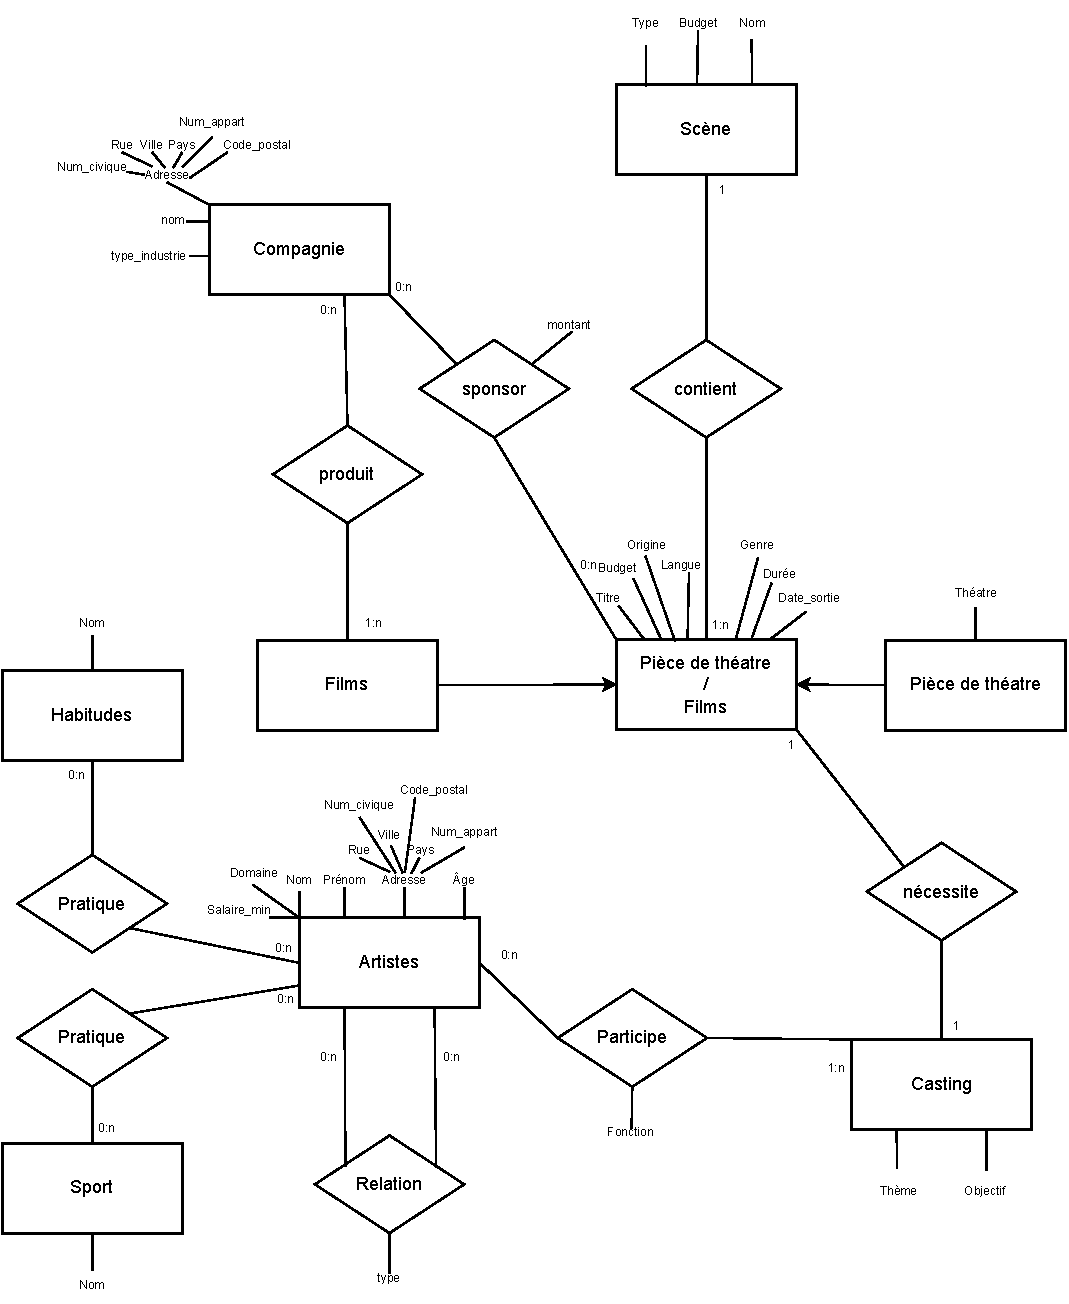
\includegraphics[scale=0.9]{../modeleEA.pdf}
\end{center}
  
\newpage

\subsection{Modèle Relationnel}


\begin{itemize}
\item \textbf{Oeuvre}(\underline{id\_oeuvre}, titre, budget,
  date\_sortie, durée, origine, langue, genre)
  
\item \textbf{Films}(\underline{\#id\_oeuvre}, \#id\_Studio)
  
\item \textbf{Pièces\_Théâtre}(\underline{\#id\_oeuvre}, théâtre)
  
\item \textbf{Scènes}(\underline{id\_scène}, titre, budget, type,
  \#id\_oeuvre)
  
\item \textbf{Adresses}(\underline{id\_adresse},no\_civique, rue,
  ville, code\_postal, pays, no\_appartement)

\item \textbf{Habitude}(\underline{id}, nom)

\item \textbf{Sport}(\underline{id}, nom)
  
\item \textbf{Artistes}(\underline{id\_artiste}, nom, prénom,
  date\_naissance, salaire\_min, domaine, \#id\_adresse)
  
\item \textbf{Casting}(\underline{\#id\_oeuvre}, objectif, thème)

\item \textbf{Casting\_Artiste}(\underline{\#id\_artiste, \#id\_oeuvre}, fonction,
  salaire, date\_debut, date\_fin)

\item \textbf{Relation}(\underline{\#id\_artiste1, \#id\_artiste2}, type\_relation)

\item \textbf{Artiste\_Sport}(\underline{\#id\_artiste, \#id\_sport})

\item \textbf{Artiste\_Habitude}(\underline{\#id\_artiste, \#id\_habitude})

\item \textbf{Compagnies}(\underline{id\_compagnie}, nom,
  type\_industrie, \#id\_adresse)
  
\item \textbf{Sponsors}(\underline{\#id\_oeuvres \#id\_compagnie},
  montant)
  
\item \textbf{Producteurs}(\underline{\#id\_oeuvres
    \#id\_compagnie})

\end{itemize}

\newpage
\subsection{Dépendances fonctionnelles}


\textbf{Oeuvre}(\underline{id\_oeuvre}, titre, budget, date\_sortie,
durée, origine, langue, genre)

\begin{itemize}
\item id\_oeuvre $\rightarrow$ titre, budget, date\_sortie, durée,
  origine, langue, genre
\end{itemize}

\vspace{2mm}
\noindent
\textbf{Addresses}(\underline{id\_adresse}, no\_civique, rue, ville, code\_postal, pays, no\_appartement)

\begin{itemize}
\item id\_adresse $\rightarrow$ no\_civique, rue, ville, code\_postal, pays, no\_appartement
\end{itemize}

\vspace{2mm}
\noindent
\textbf{Habitude}(\underline{id\_habitude}, nom)

\begin{itemize}
\item id\_habitude $\rightarrow$ nom
\item nom $\rightarrow$ id\_habitude
\end{itemize}

\vspace{2mm}
\noindent
\textbf{Sport}(\underline{id\_sport}, nom)

\begin{itemize}
\item id\_sport $\rightarrow$ nom
\item nom $\rightarrow$ id\_sport
\end{itemize}

\vspace{2mm}
\noindent
\textbf{Compagnies}(\underline{id\_compagnie}, nom, type\_industrie, \#id\_adresse)

\begin{itemize}
\item id\_compagnie $\rightarrow$ nom, type\_industrie, id\_adresse
\end{itemize}

\vspace{2mm}
\noindent
\textbf{Films}(\#\underline{id\_oeuvre}, \#\underline{id\_studio})

\begin{itemize}
\item id\_oeuvre $\rightarrow$ id\_studio
\end{itemize}

\vspace{2mm}
\noindent
\textbf{Pièce\_Théâtre}(\#\underline{id\_oeuvre}, théâtre)

\begin{itemize}
\item id\_oeuvre $\rightarrow$ théâtre
\end{itemize}

\vspace{2mm}
\noindent
\textbf{Scènes}(\underline{id\_scène}, titre, budget, type, \#id\_oeuvre)

\begin{itemize}
\item id\_scène $\rightarrow$ titre, budget, type, id\_oeuvre
\item id\_oeuvre, titre $\rightarrow$ id\_scène, type, budget
\end{itemize}

\vspace{2mm}
\noindent
\textbf{Artiste}(\underline{id\_artiste}, nom, prénom, date\_naissance, salaire\_min, domaine, \#id\_adresse)

\begin{itemize}
\item id\_artiste $\rightarrow$ nom, prénom, date\_naissance, salaire\_min, domaine, id\_adresse
\end{itemize}

\vspace{2mm}
\noindent
\textbf{Casting}(\#\underline{id\_oeuvre}, objectif, thème)

\begin{itemize}
\item id\_oeuvre $\rightarrow$ objectif, thème
\end{itemize}

\vspace{2mm}
\noindent
\textbf{Sponsor}(\#\underline{id\_oeuvre}, \#\underline{id\_compagnie}, montant)

\begin{itemize}
\item id\_oeuvre, id\_compagnie $\rightarrow$ montant
\end{itemize}

\vspace{2mm}
\noindent
\textbf{Producteur}(\#\underline{id\_oeuvre}, \#\underline{id\_compagnie})

\newpage
\noindent
\textbf{Casting\_Artiste}(\#\underline{id\_artiste}, \#\underline{id\_oeuvre}, fonction, salaire, date\_début, date\_fin)

\begin{itemize}
\item id\_artiste, id\_oeuvre $\rightarrow$ fonction, salaire, date\_début, date\_fin
\end{itemize}

\vspace{2mm}
\noindent
\textbf{Relation}(\#\underline{id\_artiste1}, \#\underline{id\_artiste2}, type\_relation)

\begin{itemize}
\item id\_artiste1, id\_artiste2 $\rightarrow$ type\_relation
\end{itemize}

\vspace{2mm}
\noindent
\textbf{Artiste\_Sport}(\#\underline{id\_artiste}, \#\underline{id\_sport})

\vspace{2mm}
\noindent
\textbf{Artiste\_Habitude}(\#\underline{id\_artiste}, \#\underline{id\_habitude})



\subsection{Normalisation}
\subsubsection*{Transformation en 1NF}
Ici rien à faire, car les tables sont déjà en 1NF: chaque attribut est
atomique.

\subsubsection*{Transformation en 2NF}
Ici rien à faire, car les tables sont déjà en 2NF: chaque attribut
non-clé ne dépend pas d'une partie de la clé.

\subsubsection*{Transformation en 3NF}
Ici rien à faire, car les tables sont déjà en 3NF:
tout attribut n'appartenant pas à la clé ne dépend pas d'un attribut non clé
\vspace{5mm}
\section{SQL}
\subsection{LDD}
Le fichier
\href{https://github.com/ZGaillard/projet_session_2935/blob/main/database/CreateUpdated.sql}{\color{blue}{\underline{CreateUpdated.sql}}}
contient la création de la base de données et des tables.

\subsection{LMD}
Le fichier
\href{https://github.com/ZGaillard/projet_session_2935/blob/main/database/Populate.sql}{\color{blue}{\underline{populate.sql}}}
contient le peuplement de la base de données. Ce fichier utilise des
procédures stockées pour generer certaines données aléatoires.
Les procédures stockées sont définies dans les fichiers 
  \href{https://github.com/ZGaillard/projet_session_2935/blob/main/database/GenCastingArtistes.sql}{\color{blue}{\underline{GenCastingArtistes.sql}}},
  \href{https://github.com/ZGaillard/projet_session_2935/blob/main/database/GenArtisteSport.sql}{\color{blue}{\underline{GenArtisteSport.sql}}}
  et
  \href{https://github.com/ZGaillard/projet_session_2935/blob/main/database/GenArtisteHabit.sql
  }{\color{blue}{\underline{GenArtisteHabit.sql}}}

  \newpage
\subsection{Requêtes}
Nous avons d'abord créer dix requêtes pour tester la base de
donnée. Ces requêtes sont dans le fichier
\href{https://github.com/ZGaillard/projet_session_2935/blob/main/database/request.sql}{\color{blue}{\underline{request.sql}}}.\n


Par la suite, nous avons créé une classe python pour exécuter des
requêtes SQL. Cette classe est dans le fichier \href{
  https://github.com/ZGaillard/projet_session_2935/blob/main/app/DBManager.py}{\color{blue}{\underline{DBManager.py}}}.
Cette classe utilise \texttt{pymssql} pour se connecter à la base de
données. Elle permet d'exécuter des requêtes simples et de récupérer
les résultats. Elle permet aussi d'exécuter des procédures stockées.\n

Durant le développement de l'application, nous avons trouvé qu'il
était plus judicieux de créer des procédures stockées pour les
requêtes qui nécessitaient des requêtes plus complexes. Ces procédures
stockées sont dans les fichiers :
\begin{itemize}
\item
  \href{https://github.com/ZGaillard/projet_session_2935/blob/main/database/DefAddAdresse.sql}{\color{blue}{\underline{DefAddAdresse.sql}}}

\item
  \href{https://github.com/ZGaillard/projet_session_2935/blob/main/database/DefAddArtist.sql}{\color{blue}{\underline{DefAddArtist.sql}}}

\item
  \href{https://github.com/ZGaillard/projet_session_2935/blob/main/database/DefAddCasting.sql}{\color{blue}{\underline{DefAddCasting.sql}}}

\item
  \href{https://github.com/ZGaillard/projet_session_2935/blob/main/database/DefAddMovies.sql}{\color{blue}{\underline{DefAddMovies.sql}}}

\item
  \href{https://github.com/ZGaillard/projet_session_2935/blob/main/database/DefAddPlays.sql}{\color{blue}{\underline{DefAddPlays.sql}}}

\item
  \href{https://github.com/ZGaillard/projet_session_2935/blob/main/database/DefGetArtistHabit.sql}{\color{blue}{\underline{DefGetArtistHabit.sql}}}
  
\item
  \href{https://github.com/ZGaillard/projet_session_2935/blob/main/database/DefGetArtistRelations.sql}{\color{blue}{\underline{DefGetArtistRelations.sql}}}
  
\item
  \href{https://github.com/ZGaillard/projet_session_2935/blob/main/database/DefGetArtistSports.sql}{\color{blue}{\underline{DefGetArtistSports.sql}}}
  
\item
  \href{https://github.com/ZGaillard/projet_session_2935/blob/main/database/DefGetArtists.sql}{\color{blue}{\underline{DefGetArtists.sql}}}
  
\item
  \href{https://github.com/ZGaillard/projet_session_2935/blob/main/database/DefGetCastingArtists.sql}{\color{blue}{\underline{DefGetCastingArtists.sql}}}
  
\item
  \href{https://github.com/ZGaillard/projet_session_2935/blob/main/database/DefGetCastings.sql}{\color{blue}{\underline{DefGetCastings.sql}}}
  
\item
  \href{https://github.com/ZGaillard/projet_session_2935/blob/main/database/DefGetCompagnies.sql}{\color{blue}{\underline{DefGetCompagnies.sql}}}
  
\item
  \href{https://github.com/ZGaillard/projet_session_2935/blob/main/database/DefGetMovies.sql}{\color{blue}{\underline{DefGetMovies.sql}}}

\item
  \href{https://github.com/ZGaillard/projet_session_2935/blob/main/database/DefGetPlays.sql}{\color{blue}{\underline{DefGetPlays.sql}}}

\end{itemize}

Tout les fichiers sql sont dans le dossier
\href{https://github.com/ZGaillard/projet_session_2935/tree/main/database}{\color{blue}{\underline{database}}}.

\subsection{}

\end{document}
